\documentclass{report}
\usepackage[utf8]{vietnam}
\usepackage[vietnamese]{babel}


% ===== Căn chỉnh lề, font chữ
\usepackage[letterpaper,top=2cm,bottom=2cm,left=3cm,right=3cm,marginparwidth=1.75cm]{geometry}


% ===== Khai báo hình ảnh
\usepackage{graphicx}
\graphicspath{ {./images/} }
\renewcommand{\listfigurename}{Danh sách hình ảnh}
\renewcommand{\listtablename}{Danh sách bảng}


% ===== Danh mục từ viết tắt
\usepackage[toc]{glossaries}
\makeglossaries
\newacronym{mvc}{MVC}{Model View Controller}
\newglossaryentry{ocopee}
{
	name=OCOPEE,
	description={Hệ thống tạo sàn thương mại điện tử cho cửa hàng}
}


% ===== Thông tin
\title{Hệ thống tạo sàn thương mại điện tử cho cửa hàng nông sản}
\author{Trần Ngọc Huy\\[1cm]{\small Giáo viên hướng dẫn: TS. Lê Thị Mỹ Hạnh}}

\date{\today}


\begin{document}
	
	
% Đánh số trang la mã
\pagenumbering{roman}
\setcounter{page}{1}


% Lời nói đầu
\chapter*{Lời nói đầu}
\addcontentsline{toc}{chapter}{Lời nói đầu}


% Cam đoan
\chapter*{Cam đoan}
\addcontentsline{toc}{chapter}{Cam đoan}


% Mục lục
\tableofcontents
\addcontentsline{toc}{chapter}{Mục lục}


% Hình ảnh
\listoffigures
\addcontentsline{toc}{chapter}{Danh sách hình ảnh}

% Bảng
\listoftables
\addcontentsline{toc}{chapter}{Danh sách bảng}


% Viết tắt 
\printglossary[title=Danh sách từ viết tắt, toctitle=Danh sách viết tắt]


\pagebreak


% ===== Nội dung đồ án =====


% Bắt đầu đánh số thứ tự arabic
\pagenumbering{arabic}
\setcounter{page}{1}

\chapter*{Mở đầu}
\addcontentsline{toc}{part}{Mở đầu}

\section*{Sứ mệnh}
\addcontentsline{toc}{section}{Sứ mệnh}
Việt Nam là một nước có truyền thống nông nghiệp. Với điều kiện tài nguyên thiên nhiên thuận lợi, nguồn nhân lực dồi
dào. Nông nghiệp đóng vai trò quan trọng trong sự phát triển kinh tế nước nhà.

Từ kỷ Hồng Bàng, trăm tộc Việt đã hợp sức tương trợ nhau. Nay, thời kì trăm hoa đua nở của nông nghiệp \& công nghệ. OCOPEE muốn tham gia vào xây dựng nền nông nghiệp Việt Nam. Với vai trò như một bộ phận thúc đẩy giao thương mua bán.
\pagebreak

\section*{Vấn đề}
\addcontentsline{toc}{section}{Vấn đề}
Tìm kiếm đầu ra cho sản phẩm là vấn đề hết sức quan trọng đối với đơn vị sản xuất. Một trong những kênh bán hàng hiệu
quả có thể kể đến đó là chương trình hội chợ, phân phối tại các cửa hàng.

Tuy nhiên, đối với các doanh nghiệp khởi nghiệp. Sản phẩm được cải tiến cập nhật thông tin liên tục. Sản lượng không đủ lớn để phân phối rộng.
\pagebreak

\section*{Giải pháp}
\addcontentsline{toc}{section}{Giải pháp}	
\gls{ocopee} cung cấp công cụ tạo trang thông tin sản phẩm riêng cho từng nhà sản xuất. Và cũng có thể chia sẽ dữ liệu sản phẩm cho các chương trình hội chợ, các cửa hàng. Các đơn vị phân phối và triễn lãm có thể tích hợp trực tiếp vào hệ thống của họ.
Ngoài ra, các sàn thương mại điện tử do OCOPEE tạo ra có khả năng tích hợp một số tính năng để tổ chức hội chợ trực tuyến.
\gls{ocopee} xác định đối tượng trực tiếp phục vụ là khách mua hàng nông sản.
- Khách hàng là người ủng hộ sử dụng nông sản chất lượng.
- Khách mua hàng tin tưởng chất lượng sản phẩm đăng tải trên hội chợ trực tuyến.
- Khách hàng dành thời gian cho các sự kiện hội chợ.
- Khách hàng cảm thấy tiện lợi trong quy trình mua hàng.
- Khách hàng được tư vấn thông tin đầy đủ về giá trị sử dụng của sản phẩm.
- Khách hàng dễ dàng tìm kiếm sản phẩm phù hợp với nhu cầu.
Nhà bán hàng là người trả tiền cho hệ thống. Thông qua việc phục vụ người mua nông sản. Hệ thống gián tiếp đem lại giá
trị cho nhà bán hàng.
- Không gian mở rộng.
- Thời gian linh hoạt.
- Khách hàng tiềm năng.
- Phù hợp với quy mô.


\part{Cơ sở lý thuyết}
\section{Node.js}
\section{PM2.js}
\section{React.js} 
\subsection{Declarative}
\subsection{Component-Based}
\paragraph{A Simple Component}
\paragraph{A Stateful Component}
\paragraph{An Application}
\subsection{Learn Once, Write Anywhere}
\section{Next.js}
\section{GraphQL}
\section{Apollo Server}
\section{MongoDB}
\subsection{What is MongoDB?}
\subsection{Summary}
\part{Phân tích thiết kế}
\chapter{Đặc tả}
\section{Giới thiệu}
\section{Mô tả chung}
\section{Yêu cầu tính năng}
\section{Yêu cầu giao diện}
\section{Yêu cầu hiêu suất}
\section{Yêu cầu thiết kế}
\section{Tiến độ và ngân sách dự tính}
\section{Phụ lục}
\chapter{Phân tích}
\section{Vai trò}
\section{Hoạt động}
\section{Phân quyền}
\section{Resources of the system}
\section{Goals}
\section{Features}
\section{Phân quyền}
\subsection{Owner}
\subsection{Seller}
\chapter{Thiết kế}
\section{Usecase Diagram}
\section{Class Diagram}
\section{Activity Diagram}
\section{Kiến trúc máy chủ}
\section{Kiến trúc ứng dụng}
\section{DevOps}
\subsection{Environments definition}
\subsubsection{Development}
\subsubsection{Staging}
\subsubsection{Production}
\part{Triển khai và đánh giá}
\chapter{Triển khai}
\section{Requirement}
\subsection{Fundamental}
\subsection{High Level Framework}
\section{Guide}
\section{Sources}
\subsection{Github ocopee respository}
\subsection{Github gateway respository}
\subsection{Github accounts respository}
\subsection{Github docs respository}
\subsection{Github sellers respository}
\subsection{Installing and setting}
\subsection{Run server locally}
\subsubsection{Backend}

%\begin{figure}[h]
%	\caption{State diagram}
%	\centering
%	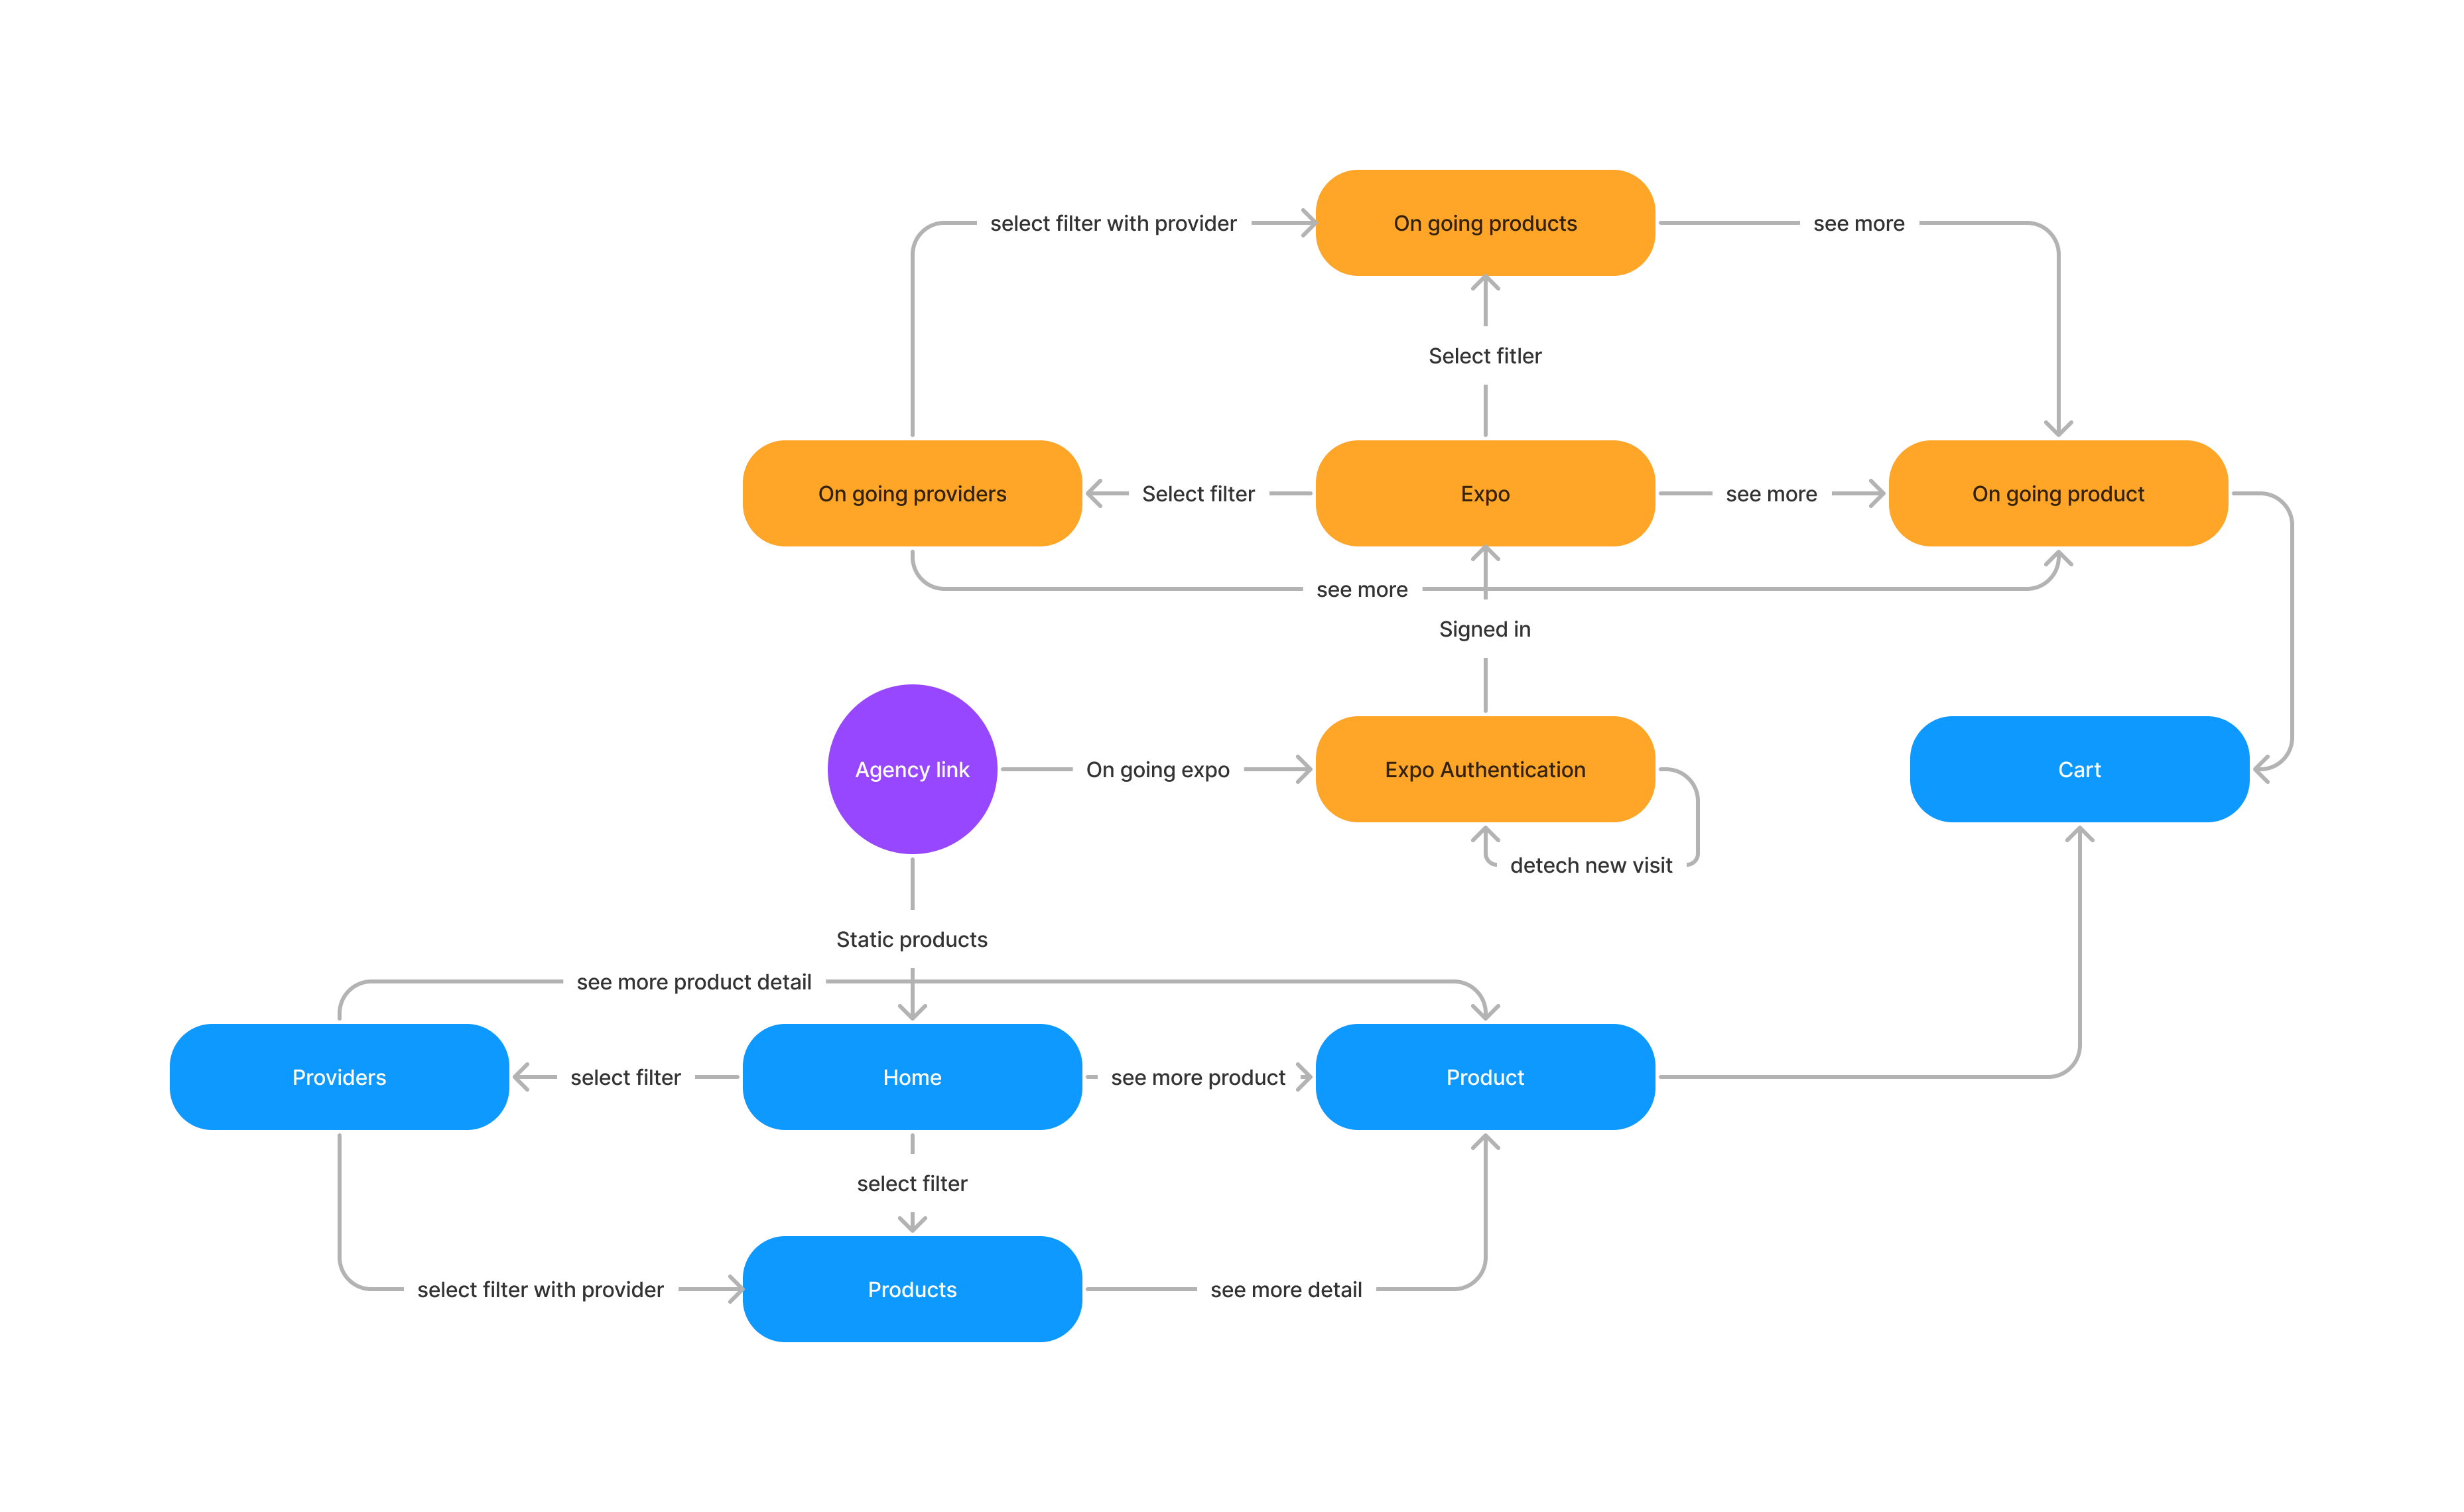
\includegraphics[width=\textwidth]{./images/state.png}
%	\label{fig:state}
%\end{figure}

\part*{Kết luận và hướng phát triển}
\chapter{Kết quả đạt được}
\chapter{Những vấn đề hạn chế}
\chapter{Hướng phát triển}

% Tham khảo
\bibliographystyle{alpha}
\bibliography{website}
\end{document}